\documentclass[letterpaper]{article}

\usepackage[mmddyy]{datetime}
\usepackage[margin=1.25in]{geometry}
\usepackage{fancyhdr}
\usepackage{amsmath}
\usepackage{amssymb}
\usepackage{graphicx}

\usepackage{listings}
\usepackage{color}

\definecolor{codeblue}{rgb}{0.2039, 0.5961, 0.8588}
\definecolor{codegreen}{rgb}{ 0.3451, 0.8392, 0.5529}
\definecolor{codedark}{rgb}{  0.2039, 0.2863, 0.3686}
\definecolor{backcolour}{rgb}{0.9176, 0.9255, 0.9333}
\definecolor{codepink}{rgb}{0.9804, 0.5490, 0.7725}

\lstdefinestyle{mystyle}{
    backgroundcolor=\color{backcolour},
    commentstyle=\color{codegreen},
    keywordstyle=\color{codeblue},
    numberstyle=\tiny\color{codedark},
    stringstyle=\color{codepink},
    basicstyle=\footnotesize,
    basicstyle=\footnotesize\fontfamily{\ttdefault}\selectfont,
    breakatwhitespace=false,
    breaklines=true,
    captionpos=b,
    keepspaces=true,
    numbers=left,
    numbersep=5pt,
    showspaces=false,
    showstringspaces=false,
    showtabs=false,
    tabsize=2
}

\lstset{style=mystyle}

\pagestyle{fancy}
\fancyhf{}
\rhead{Cort Breuer}
\chead{\today}
\lhead{ENGRD 2700}
\rfoot{\thepage}

\begin{document}

\vspace*{6pt}

\noindent \textbf{\huge{Problem Set 5}}

\bigskip

\section*{Question 1}

Joint density function given by $f_{X, Y}(x, y)=\left\{\begin{array}{ll}{k(2 y+x y)} & {\text { if } 0 \leq x \leq 1 \text { and } x \leq y \leq 1} \\ {0} & {\text { otherwise. }}\end{array}\right$

\subsection*{Part A}

$$\int \int f_{X,Y} (x, y) dx dy = 1$$

$$\int_0^1 \int_x^1 k(2y+xy) dy dx + \int \int 0 dx dy = 1$$


$$\int_0^1 \int_x^1 [ 2ky + kxy ] dy dx = 1$$

$$\int_0^1 [ ky^2 + \frac{1}{2} kxy^2 ] \Big|_x^1 dx = 1$$

$$\int_0^1 [ k - kx^2 + \frac{1}{2} kx - \frac{1}{2} kx^3] dx = 1$$

$$[ kx - \frac{1}{3} kx^3 + \frac{1}{4} kx^2 - \frac{1}{8} kx^4 ] \Big|_0^1 = 1$$

$$k[1 - 0] - \frac{1}{3}[k - 0] + \frac{1}{4}[k - 0] - \frac{1}{8}[k - 0] = 1$$

$$k - \frac{k}{3} + \frac{k}{4} - \frac{k}{8} = 1$$

$$k \frac{19}{24}= 1$$

$$k = \frac{24}{19}$$

\subsection*{Part B}

$$\text{Marginal PDF of } X \ f_X(x) = \int f_{X, Y}(x, y) dy$$

$$f_X(x) = \int_0^1 k(2y + xy) dy = k(y + \frac{1}{2} xy^2) \Big|_0^1$$

$$f_X(x) = k \Big[ (1 + \frac{1}{2} x) - (0 + \frac{1}{2} 0) \Big] = \frac{24}{19} [1 + \frac{1}{2} x]$$

$$f_X(x) = \frac{24}{19} + \frac{12}{19} x$$

$$\text{Marginal PDF of } X \ f_X(x) = \begin{cases} \frac{24}{19} + \frac{12}{19} x & 0 \leq x \leq 1 \\ 0 & \text{otherwise} \end{cases}$$

\subsection*{Part C}

$$f_{X|Y} (x|y) = \frac{f_{X,Y}(x,y)}{f_Y(y)}$$

$$f_Y(y) = \int f_{X, Y}(x, y) dx = \int_0^y k(2y + xy) dx$$

$$f_Y(y) = k(2yx + \frac{1}{2} x^2y) \Big|_0^y = \frac{24}{19} (2y^2 + \frac{1}{2} y^3)$$

$$f_{X|Y} (x|y) = \frac{\frac{24}{19}(2y + xy)}{\frac{24}{19} (2y^2 + \frac{1}{2} y^3)} = \frac{2 + x}{2y + \frac{1}{2} y^2)}$$

$$f_{X|Y} (x|\frac{1}{4}) = \frac{2 + x}{\frac{1}{2} + \frac{1}{32}} = \frac{2 + x}{\frac{17}{32}} = \frac{64 + 32x}{17}$$

$$f_{X|Y} = \begin{cases} \frac{64 + 32x}{17} & 0 \leq x \leq \frac{1}{4} \\ 0 & \text{otherwise} \end{cases}$$

\newpage

\section*{Question 2}

Lifetime X and Y of two batteries given by joint PDF $f_{X,Y}(x, y) = \begin{cases} 8e^{-4x}e^{-2y} & x, y \geq 0 \\ 0 & \text{otherwise} \end{cases}$

\subsection*{Part A}

$$P(X, Y \geq 2) = \int_2^{\infty} \int_2^{\infty} 8e^{-4x}e^{-2y} dx dy$$

$$P(X, Y \geq 2) = \int_2^{\infty} -2e^{-4x}e^{-2y} \Big|_2^{\infty} dy = \int_2^{\infty} -2e^{-\infty}e^{-2y} + 2e^{-8}e^{-2y} dy$$

$$P(X, Y \geq 2) = \int_2^{\infty} 2e^{-8}e^{-2y} dy = -e^{-8}e^{-2y} \Big|_2^{\infty}$$

$$P(X, Y \geq 2) = -e^{-8}e^{-\infty} + e^{-8}e^{-4} = e^{-12} = 6.14 \cdot 10^{-6}$$

\subsection*{Part B}

$$f_X(x) = \int_0^{\infty} 8e^{-4x}e^{-2y} dy = -4e^{-4x}e^{-2y} \Big|_0^{\infty} = 4e^{-4x-4} \text{for } x \geq 0$$

$$f_Y(y) = \int_0^{\infty} 8e^{-4x}e^{-2y} dx = -2e^{-4x}e^{-2y} \Big|_0^{\infty} = 2e^{-2y-8} \text{for } x \geq 0$$

\subsection*{Part C}

E[XY] =

\subsection*{Part D}

\subsection*{Part E}

\newpage

\section*{Question 3}

$$\begin{array}{c|c|ccc}{} & {} & {s} & {} & {} \\ \hline f_{R, S(r, s)} & {0} & {1} & {2} \\ \hline 0 & {0} & {0.25} & {0.15} \\ {1} & {0.20} & {0.10} & {0.10} \\ {2} & {0.10} & {0.05} & {0.05} \\ \hline\end{array}$$

\subsection*{Part A}

\subsection*{Part B}

\subsection*{Part C}

\newpage

\section*{Question 4}

$$\text{Joint PDF given by } f_{X|Y}(x, y) = \begin{cases} 2ye^{-y(2+x)} & x, y \geq 0 \\ 0  & \text{otherwise} \end{cases}$$

$$f_{X|Y}(x|y) = \frac{f_{X,Y}(x, y)}{f_Y(y)}$$

$$f_Y(y) = \int_0^{\infty} 2ye^{-y(2+x)} dx = -2 \int_0^{\infty} e^u dx \text{ with } u = -y(2+x)$$

$$f_Y(y) = -2 e^u \Big|_0^{\infty} = -2 e^{-y(2+x)} \Big|_0^{\infty}$$

$$f_Y(y) = -2 e^{-y(2+ \infty)} + 2 e^{-y(2+0)} = 2 e^{-2y}$$

$$f_{X|Y}(x|y) = \frac{f_{X,Y}(x, y)}{f_Y(y)} = \frac{2ye^{-y(2+x)}}{2 e^{-2y}}$$

$$f_{X|Y}(x|y) = \frac{y e^{-2y} e^{-yx}}{e^{-2y}} = y e^{-yx}$$

$$f_{X|Y}(x|y) = \begin{cases} y e^{-yx} & x, y \geq 0 \\ 0 & \text{otherwise} \end{cases}$$

\newpage

\section*{Question 5}

\begin{lstlisting}[language=R]
    Bwages <- read_csv("Bwages.csv")
\end{lstlisting}

\subsection*{Part A}

\begin{lstlisting}[language=R]
    ggplot(data = Bwages) + geom_histogram(mapping = aes(x = wage), binwidth = 3) + xlab("Wages") + ylab("Count") + ggtitle("Wage Histogram")
\end{lstlisting}

\begin{center}
    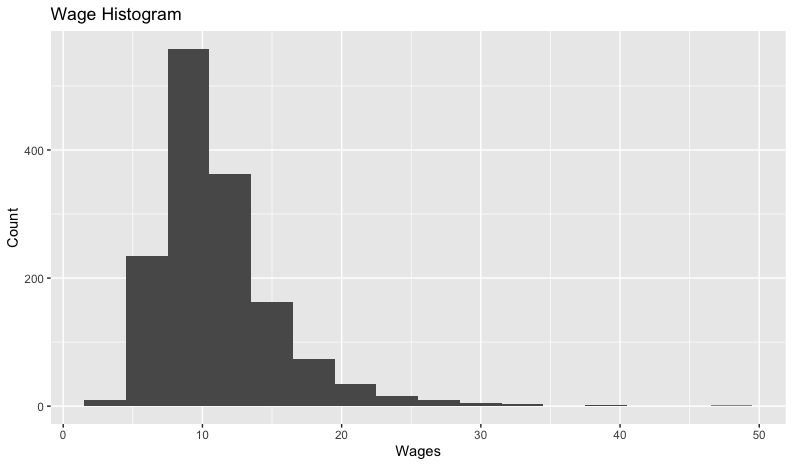
\includegraphics[width=5in]{wageHistogram.png}
\end{center}

\subsection*{Part B}

\begin{center}
    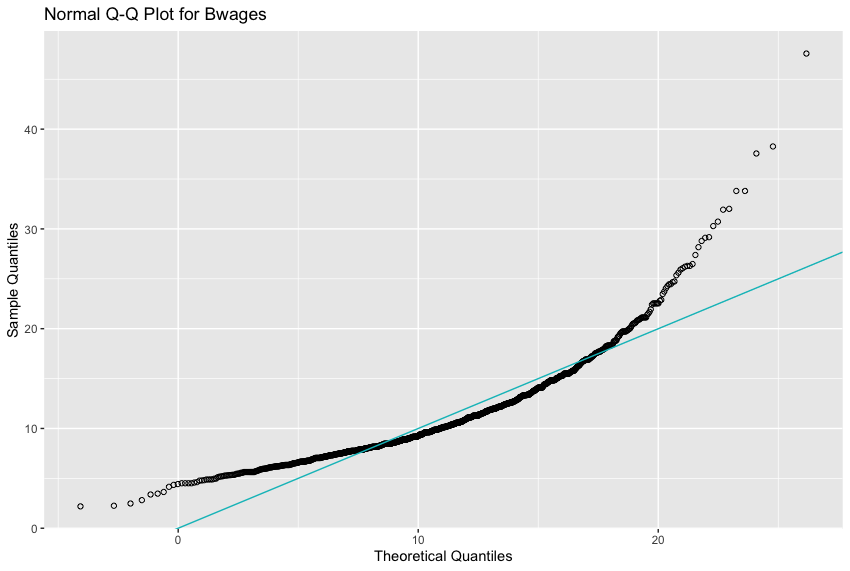
\includegraphics[width=5in]{QQPlot.png}
\end{center}

\begin{lstlisting}[language=R]
    n = length(Bwages$wage)
    qi = (1:n - 0.5)/n
    mu = mean(Bwages$wage)
    sigma = sd(Bwages$wage)

    x = qnorm(qi, mu, sigma)
    y = sort(Bwages$wage)
    wages <- tibble(x, y)

    ggplot(data = wages) + geom_point(mapping = aes(x = x, y = y), shape = 1) + geom_abline(intercept = 0, slope = 1) + xlab("Theoretical Quantiles") + ylab("Sample Quantiles") + ggtitle("Normal Q-Q Plot for Bwages")
\end{lstlisting}

\subsection*{Part C}

The normal distribution looks to be a poor fit of the wage data provided. The long tails on both the left and right indicate that the normal distribution is especially poor at modeling edge points. This is likely due to the combined effect of wages never going negative even though the normal distribution does (seen on the axes) and on the right side especially high wages that do not follow the normal distribution well.

\subsection*{Part D}

Fit a lognormal distribution to Bwages, using $X \sim \text{Lognormal} (\mu, \sigma^2)$ with PDF of:

$$f(x) = \frac{1}{x \sigma \sqrt{2 \pi}} e^{-(ln(x) - \mu)^2 / (2 \sigma^2)} \text{when } x > 0$$

\begin{center}
    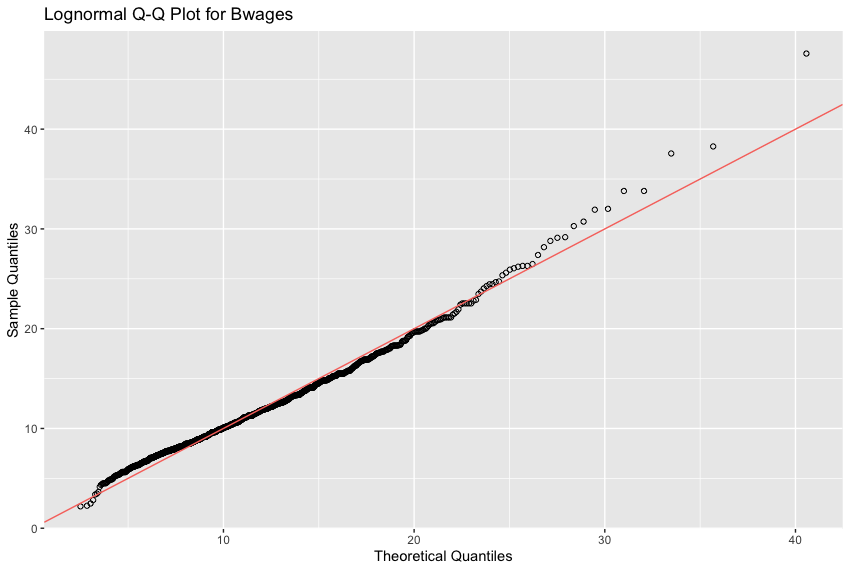
\includegraphics[width=5in]{LogQQPlot.png}
\end{center}

\begin{lstlisting}[language=R]
    meanlog <- 2.31
    sdlog <- .41

    n = length(Bwages$wage)
    qi = (1:n - 0.5)/n

    x = qlnorm(qi, meanlog, sdlog)
    y = sort(Bwages$wage)
    wages <- tibble(x, y)

    ggplot(data = wages) + geom_point(mapping = aes(x = x, y = y), shape = 1) + geom_abline(intercept = 0, slope = 1, color = "#F8766D") + xlab("Theoretical Quantiles") + ylab("Sample Quantiles") + ggtitle("Lognormal Q-Q Plot for Bwages")
\end{lstlisting}

\subsection*{Part E}

\end{document}
